
% Preamble
\documentclass[12pt, letterpaper]{article}
\title{Chapter 4 - Traveling Waves - Notes}
\author{Jordan Tucker}
\date{April 6, 2026}
% Packages
\usepackage{amsmath}
\usepackage{parskip}
\usepackage{tabularx}
\usepackage{graphicx}
\usepackage{enumitem}
\usepackage{hyperref} %LaTeX package to import graphics
\graphicspath{{images/}} %configuring the graphicx package

% Document
\begin{document}
    \maketitle
    \section{Traveling Waves}\label{sec:traveling-waves}

    \subsection{Traveling Waves}\label{subsec:traveling-waves}
    Waves represented by functions/solutions in the form $u(x,t) = f(x-ct)$ are called
    \textit{traveling waves}, where $f$ describes the shape of the wave and $|c|$ is the speed of
    the wave.

    If $c<0$ then the wave moves in the negative $x$ direction.
    If $c>0$ then the wave moves in the positive $x$ direction.

    It is assumed that $f$ is not constant and $c$ is not 0 to represent movement through a medium.

    \textbf{Example:} $e^{-(x-5t)^2}$ is moving in the positive $x$ direction with speed 5.
    
    A \textbf{traveling wave solution} of a PDE is a solution of the differential equation which
    has the form $u(x,t) = f(x-ct)$.
    You can begin finding traveling wave solutions by assuming $u(x,t) = f(x-ct)$ and then
    determining which functions $f$ and constants $c$ yield a solution to the differential equation.
    \\
    \newpage
    \textbf{Example:} We want to find a traveling wave solution to the wave equation
    \[
        u_{tt}=au_{xx},\quada>0 \ \text{constant}
    \]
    Assuming that $u(x,t) = f(x-ct)$, we can use the chain rule.
    \[
        \begin{aligned}
            u_t(x,t) &= f'(x-ct)(x-ct)_t = -cf'(x-ct) \\
            u_x(x,t) &= f'(x-ct)(x-ct)_x = f'(x-ct)
        \end{aligned}
    \]
    And we can use the chain rule again.
    \[
        \begin{aligned}
            u_{tt}(x,t) &= f''(x-ct)(x-ct)_t = c^{2}f''(x-ct) \\
            u_{xx}(x,t) &= f''(x-ct)(x-ct)_x = f''(x-ct)
        \end{aligned}
    \]
    We can then plug our results back into the wave equation and re-arrange so it looks nice.
    \[
        \begin{aligned}
            u_{tt} &= au_{xx} \\
            c^{2}f''(x-ct) &= af''(x-ct) \\
            c^{2}f''(x-ct) - af''(x-ct)& = 0\\
            f''(x-ct)(c^{2}-a)=0
        \end{aligned}
    \]
    When can then sub in $z=x-ct$
    \[
        f''(z)(c^{2}-a)=0
    \]
    In order for the above to be satisfied, $c^2=a$ and $f$ must be twice differentiable, or $f''=0$
    (meaning $f$ must be some linear function $f(z)=A+Bz$).
    Example solutions:
    \[
        \begin{aligned}
            u(x,t) &= f(x- \sqrt{a} t) \\
            u(x,t) &= f(x+ \sqrt{a} t) \\
            u(x,t) &= sin(x- \sqrt{a} t)\\
            u(x,t) &= A+B(x-ct)
        \end{aligned}
    \]

    \subsection{Wave fronts and pulses}

    A traveling wave represented by $u(x,y)$ is said to be a \textit{wave front} if for any fixed t,
    \[
        u(x,t) \rightarrow k_1 \ \text{as} \ x \rightarrow -\infty, \quad u(x,t)\rightarrow k_2 \
        \text{as} \ x\rightarrow \infty
    \]
    where $k_1$ and $k_2$ are constants.
    $k_1$ and $k_2$ do not have to be equal.
    If $k_1=k_2$, then the wave front is called a \textit{pulse}.
    A \textit{pulse} temporarily changes the value of $u$ at position $x$ before it settles back to
    its original value.

    A physical example could be a cold front in weather.
    Temperatures ahead of the disturbance can be a relatively constant $k_1$, and the temperatures behind
    the disturbance can be around $k_2$.
    The disturbance can cause a sudden drop in the temperature (sometimes more than 30 degrees F)
    from $k_1$ to $k_2$.

    \begin{figure}[h]
        \centering
        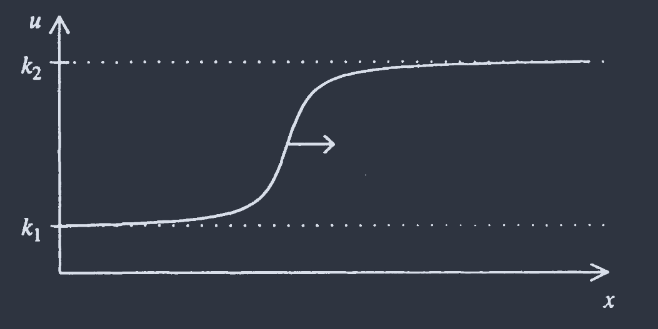
\includegraphics[width=0.75\textwidth]{wavefront}
        \caption{The profile of a wave front at time $t$.}
    \end{figure}
    
    \subsection{Wave trains and dispersion}\label{subsec:wave-trains-and-dispersion}
    A traveling wave which can be written in the form
    \[
        u(x,t) = Acos(kx-\omega t)\quad  or \quad u(x,t)=Acos(kx+ \omega t)
    \]
    where $A \neq 0$, $k>0$ and $\omega > 0$ are constants is called a \textit{wave train}.
    Rewriting the $u(x,t)$ as
    \[
        u(x,t) = Acos\left[ k \left(x- \frac{\omega}{k} t \right) \right]
    \]
    shows us that it is a traveling wave with the shape $f(z)=Acos(kz)$ and moving with the speed
    $c=\frac{\omega}{k}$
    More generally, wave trains are represented as $u(x,t) = f(kx-\omega t)$ where $f(z)$ is a
    periodic function.

    \begin{enumerate}[label=\alph*)]
    \item $k$ is called the \textit{wave number} and represents the number of cycles on this period
    wave that appears in a window of length $2\pi$ on the $x$-axis.
    \item The number $\omega$ is called the circular frequency and represents the number of cycles
    of the wave that pass by any fixed point $x$ on the $x$-axis during a time interval of $2 \pi$.
    \end{enumerate}

    A PDE may have solutions that are wave trains but not for every possible value of $k$ and
    $\omenga$.

    To find which wave numbers and frequencies are permitted, one can substitute the form of a wave
    train such as $u(x, t) = Acos(kx - \omega t)$ into the differential equation and reduce it to a
    relationship between $k$ and $\omega$.
    This relationship is called a \textit{dispersion} relation and indicates
    which values of $k$ and $\omega$ may be selected in order for $u(x, t)$ to be a wave train
    solution.

    A partial differential equation which has wave train solutions is said to be \textit{dispersive}
    if waves trains of different frequencies $\omega$ propagate through the medium with different
    speeds.

    A PDE is dispersive only if its phase velocity $v_p = \frac{\omega}{k}$ is not constant,
    meaning $\frac{d^2\omega}{dk^2} \neq 0$.
    If all wave trains travel at the same speed regardless of their $\omega$, the PDE is not
    dispersive.
\end{document}